%! Author = mboehme
%! Date = 23.02.2023

\section{Technische Umsetzung}\label{sec:technische-umsetzung}
%Entwicklung fängt schon vorher an.
\subsection{Prototyp}\label{subsec:prototyp}
Basierend auf dem Mockup ~\ref{fig:Mockup} wurde ein Prototyp erstellt, welcher testen sollte, ob Grundfunktionalitäten wie die Terminbuchung und die Darstellung der Termine funktionieren.
Dies wurde mithilfe von vuejs aufgesetzt.
\newline
Der Prototyp funktionierte wie erwartet und konnte somit als Grundlage für die Weiterentwicklung dienen.
\subsection{Benutzte Hardware und Software}\label{subsec:benutzte-hardware-und-software}
\newline
Die Hardware ist ein Philips~\cite{10BDL4551T/00} Bildschirm.
Dieser Bildschirm ist ein 10 Zoll (ca. 25 cm diagonal) Touchscreen.
Es hat eine Auflösung von 1280x800 Pixeln und benutzt Android als Betriebssystem.
\newglossaryentry{Digital Signage}{name={Digital Signage}, description={Digital Signage ist eine ferngesteuerte, digitale Anzeige. Sie wird meistens in öffentlichen Räumen, wie zum Beispiel Flughäfen, Einkaufszentren oder Bahnhöfen, verwendet.}}
Der Bildschirm ist für Digital Signage gedacht und kann so auch als solches verwendet werden.
\newglossaryentry{SICP}{name=SICP, description={SICP steht für Serial (Ethernet) Interface Communication Protocol.
SICP ist ein Protokoll, welches es ermöglicht, mit dem Bildschirm direkt zu kommunizieren, ohne mit dem Android Betriebssystem zu interagieren.}}
Die eingebauten RGB LED Strips können per~\gls{SICP} angesteuert werden.
Dafür wird Dory-node.js genutzt, um auf einen lokalen Server zu hören und die Anfragen an den Bildschirm weiterzuleiten.
Es wird dafür keine Internetverbindung benötigt.
Dokumentationen für SICP öffentlich schwierig zu finden.
Befehle werden als Hexadezimal Werte geschrieben und an den Bildschirm gesendet.
%Quellenangabe
Die Verschlüsselung passiert, indem ein XOR aller vorausgehenden Bytes genommen und als Prüfsumme mitgegeben wird.
Diese Verschlüsselung ist von Phillips definiert.
Sie soll lediglich verhindern, dass jemand versehentlich falsche Befehle an den Bildschirm sendet.
\newline
\newline
\newglossaryentry{IDE}{name=IDE, description={Eine IDE ist eine Entwicklungsumgebung, die es ermöglicht, Software zu entwickeln.}}
Zur Entwicklung der Anwendung, wird eine~\gls{IDE} benötigt.
Als JavaScript Framework wird Vue.js verwendet, da es sich um eine Single Page Application handelt und Vue.js darauf spezialisiert ist.
\newline
\newglossaryentry{Node.js Server}{name={Node.js Server}, description={Ein Node.js Server ist ein Server, der auf Node.js basiert und JavaScript Code ausführt.}}
Um eine Kommunikation zwischen der Anwendung und dem Bildschirm zu ermöglichen, wird ein~\gls{Node.js Server} benötigt.
Dieser wird per Dory-node.js lokal gehostet.
\newglossaryentry{NPM}{name=NPM, description={NPM steht für Node Package Manager.}}
\newline
Damit die Authentifizierung funktioniert und Prozesse, wie das Einloggen, vereinfacht werden können, wird microsoft-mgt~\cite{Microsoft-mgt-npm} als~\gls{NPM} Package verwendet.
Dies beinhaltet das Microsoft Graph Toolkit~\cite{Microsoft-Graph-Toolkit}, welches alle Microsoft Graph API Komponenten enthält.
\newline
Für eine hohe Kompatibilitätsgewährleistung, wird Babel~\cite{Babel} und Webpack~\cite{Webpack} verwendet.
Babel stellt sicher, dass der Code in allen Browsern lauffähig ist und Webpack sorgt dafür, dass die Anwendung schnell lädt.
\newline
Um eine ordentliche Versionierung zu betreiben, wird Git, welches ein dezentrales Versionskontrollsystem ist, genutzt.
Es ermöglicht, Änderungen an Dateien zu verfolgen und zu verwalten.
Dies wird in Zusammenhang mit GitLab verwendet, da dies der derzeitige, etablierte Standard der DooH media GmbH ist.
\newline
\newglossaryentry{Linter}{name=Linter, description={Ein Linter ist ein Programm, das es ermöglicht, Code auf Fehler zu prüfen.}}
Zum Vermeiden von schlechter Codequalität und syntaktischen Fehlern, die der Compiler nicht erkennen kann, wird EsLint~\cite{EsLint} verwendet.
EsLint ist ein~\gls{Linter}, der es ermöglicht, JavaScript Code zu analysieren und zu formatieren.
Da Testfälle bei JavaScript Projekten nicht vor der Ausführung der Anwendung möglich sind, ist es wichtig, dass der Code einheitlich ist und keine syntaktischen Fehler enthält.
Deshalb achtet EsLint auf die Einhaltung von Regeln, damit erst gar keine Fehler entstehen, die durch falsche Syntax entstehen.
Beispielsweise wird überprüft, ob Variablen, welche deklariert werden, auch verwendet werden.
\newline
\newline
\subsection{Grobe Planung}\label{subsec:grobe-planung}
\newglossaryentry{deployen}{name=deployen,description={Eine Anwendung zu deployen bedeutet, sie auf einem Server zu installieren und zu konfigurieren, sodass sie für den Benutzer verfügbar ist.}}
Die Software wird als eine Azure App deployt (~\gls{deployen}).
\newglossaryentry{localhost}{name=localhost,description={Die lokale Adresse des Computers, auf dem die Anwendung läuft.}}
\newglossaryentry{cookie cache}{name=cookie cache,description={Ein Cookie ist eine kleine Textdatei, die von einem Webserver auf dem Computer des Benutzers gespeichert wird. Cookies werden verwendet, um Informationen über den Benutzer zu speichern.}}
Diese lässt ~\gls{localhost} Verbindungen zu und gibt einem die Möglichkeit das ganze als Single Page Application zu entwickeln, mit einem lokalen ~\gls{cookie cache} für den eingeloggten Account.
Deshalb agiert die Anwendung erstmal nur als ein Gerüst, welches darauf wartet, dass der Benutzer sich einloggt.
Sobald sich der Benutzer einloggt, wird die Anwendung mit den Daten des Benutzers gefüllt.
Somit ist keine Individualisierung der Seite für verschiedene Nutzer notwendig.
\newline
\newglossaryentry{Azure AD}{name=Azure AD,description={Azure Active Directory ist ein Verzeichnisdienst, der von Microsoft entwickelt wurde.}}
Der wichtigste Faktor für die Entscheidung, die Microsoft Graph API zu nutzen war, dass mithilfe von ~\gls{Azure AD}, die Authentifizierung und Autorisierung von Benutzern erlaubt.
\newglossaryentry{Dory-node.js}{name=Dory-node.js,description={Dory-node.js ist eine Android App, die es ermöglicht, node.js Server auf einem Android Gerät zu hosten.}}
Es wird, lokal, mithilfe von~\gls{Dory-node.js} gehostet.
\newline
%Das Wort "Player" einführen
\newglossaryentry{Player}{name=Player,description={Ein Player ist ein Digital Signage Gerät, welches Inhalte anzeigt.}}
Der ~\gls{Player} benötigt auf der OMS den Content-Typen \("\)Web\("\),
\newline
mit der URL: \("\)http://localhost:3000/content\("\).
Diese Seite wird dann lokal vom Player aufgerufen, worauf der Dory-node.js Server antwortet und die tatsächliche Seite anbietet, die lokal auf dem Bildschirm liegt.
%Bitte im Soll-Zustand einführen was oAuth ist
So ist die URL durchgehend, auf allen Geräten identisch, damit die OAuth 2.0 URI Bedingungen erfüllt sind.
\newline
\newline
\newline
\pagebreak


\subsection{Iterative Entwicklung der groben Planung}\label{subsec:iterative-entwicklung-der-groben-planung}
Es wurde eine Azure App erstellt, die die Authentifizierung der Anwendung und des Benutzers übernimmt.
\newline

Dort wird der Benutzer eingeloggt und die Anwendung leitet ihn auf die Seite weiter, die er vorher besucht hat, welche in diesem Fall, die Raumbuchungsseite ist.
\newline
Es wurde jede Woche Rücksprache mit dem Kunden gehalten, um die Anforderungen zu besprechen und zu erfüllen.
Aber auch intern wurde Rücksprache gehalten, was denn sinnvoll ist und was nicht.
\newline
%Iterative Entwicklung mit Kundenentwicklung. Vllt eigenes Kapitel
So wurde jede Woche die Anwendung weiterentwickelt und verbessert.
Teilweise wurden auch neue Features hinzugefügt, die nicht initial erwünscht, aber sinnvoll waren.
Manche Features wurden auch wieder entfernt, da sie nicht sinnvoll waren oder von anderen Features abgedeckt wurden.
\newline
%Ablauf der Entwicklung
\newline
\subsection{Ablauf der Entwicklung}\label{subsec:ablauf-der-entwicklung}
Nachdem der erste Prototyp fertig war und Rücksprache gehalten wurde, wurde angefangen die Anwendung zu entwickeln.
Design und Funktionalität wurden dabei partiell parallel entwickelt, wobei die Funktionalität immer Priorität hatte.
In über 95 Commits wurden die Änderungen an der Anwendung festgehalten.
\newline
Es wurde ein Testgerät benötigt, um die Anwendung zu testen.
Ein Phillips 10BDL4551T/00 Bildschirm wurde dafür an die Wand gehängt und mit dem Internet verbunden.
Die Internetverbindung ist notwendig, um die Rest-Anfragen zwischen der Anwendung und der Microsoft Graph API zu ermöglichen.
Es wurde so eingerichtet, wie es auch beim Kunden laufen soll.
\newline
Die Anwendung wurde täglich aktiv genutzt, um so Fehler zu finden und Feedback zu geben.
Das Feedback wurde dann evaluiert.
Solche explorativen Tests sind sehr wichtig, um Intuitivität und Benutzerfreundlichkeit zu gewährleisten.
Es war einerseits hilfreich, um vorgesehene Abläufe zu testen, andererseits aber auch um Fehler zu finden, die nicht vorgesehen waren, indem Monkey Testing~\cite{Monkey-Testing-Book1} betrieben wurde.
\newline
\subsection{Rest-Anfragen}\label{subsec:rest-anfragen}
Mithilfe der oDatav4 (~\cite{oData}) API wurden die Daten aus der jeweiligen Microsoft Datenbank im Voraus gefiltert, um so nicht notwendige Daten zu vermeiden und die Performance drastisch zu erhöhen, als auch Datenvolumen zu sparen.
Die Daten wurden dabei im JSON Format zurückgegeben.
Die oData v4 API verhält sich dabei wie eine SQL Datenbank, wobei die Daten in Tabellen gespeichert sind.
\newline
Um sicherzustellen, dass die Anfragen ISO 8601 konform sind, wird die Zeitzone bei jeglichen Anfragen mit angegeben.
%Satz zu lang, umformieren
Es wurden die Klauseln \("\$\)filter\("\) und \("\$\)top\("\) verwendet, um nur Termine für den aktuellen und nächsten Tag zu erhalten und dies einzuschränken auf die top 300 Termine, falls jemand versucht das System zu überlasten.
Eine Sortierung ist nicht notwendig, da die Termine bereits nach Startzeit sortiert sind.
Hier sieht man die oData v4 API Anfrage, die an die Microsoft Graph API gesendet wird:
\newline
%add Fix code listing and remove .
\begin{lstlisting}[language=JavaScript,label={lst:JavaScript oData v4 API Anfrage}]
     let url =  "https://graph.microsoft.com/v1.0/me/findMeetingTimes/?$filter=start/dateTime" +  "ge"  + "${todayDate} and end/dateTime le ${tomorrowDate}&$top=300";
\end{lstlisting}
\subsubsection{Abfrageoptimierung}\label{subsubsec:abfrageoptimierung}
\("\)https://graph.microsoft.com/v1.0/me/findMeetingTimes/\("\) ist die URL der Microsoft Graph API.
Des Weiteren kommuniziert sie, welche API, spezifisch angesprochen werden soll.
Da die Termine für den aktuellen und nächsten Tag benötigt werden, wird die \("\)FindMeetingTimes\("\) verwendet, welche die Kalender API verwendet.
Mit dem \("\)me\("\) wird der aktuelle Benutzer mitgegeben.
Dieser wird automatisch vom Microsoft Graph erkannt.
\newglossaryentry{Query Parameter}{name=Query Parameter,description={Query Parameter sind Parameter, die an eine URL angehängt werden können, um die Anfrage zu verfeinern.}}
Ab dem Fragezeichen werden die Query Parameter übergeben.
Die Antwort der Anfrage, im Teil der URL, vor dem Fragezeichen, werden durch die Query Parameter auf die benötigten Daten gefiltert.
\newline
Mit \("\)start/dateTime\("\) + \("\)ge\("\) + \("\){todayDate}\("\) wird der Startzeitpunkt des Termins mit dem heutigen Datum verglichen.
Es wird geprüft, ob der Startzeitpunkt des Termins nach dem heutigen Datum liegt.
Das \("\)ge\("\) steht für \("\)greater than or equal to\("\) und bedeutet, dass der Startzeitpunkt des Termins nach oder gleich dem heutigen Datum liegt.
Dies wird eigentlich für mathematische Vergleiche verwendet, aber es funktioniert auch für Strings, da jeder Charakter einen ASCII Wert hat.
\newline
Somit erhalten wir nur Daten zurück, die heute oder in der Zukunft liegen.
\newline
Mit \("\)end/dateTime\("\) + \("\)le\("\) + \("\) {tomorrowDate}\("\) wird der Endzeitpunkt des Termins mit dem morgigen Datum verglichen.
Letzten Endes erhalten wir nur Termine zurück, die heute oder morgen stattfinden.
Die Verarbeitung dieser Daten erfolgt ISO 8601 konform.
Sobald diese jedoch angezeigt werden, wird darauf geachtet, dass es die lokale Zeitzone ist.
\newline
%Probleme gehören eigentlich woanders hin
\subsubsection{Probleme}\label{subsubsec:probleme}
Es wurden im Voraus Befehle im Microsoft Graph Explorer~\cite{Microsoft-Graph-Explorer} ausgeführt, um zu testen, ob die Anfrage funktioniert und ob die Daten in der gewünschten Form zurückgegeben werden.
Jedoch hat sich herausgestellt, dass der Microsoft Graph Explorer nicht korrekt funktioniert und teilweise Befehle nicht entgegennimmt, die laut Microsoft Dokumentation funktionieren sollten.
Evident ist dies, da die Anwendung korrekt funktioniert und die REST API Anfragen korrekt funktionieren und auch im Request-Response Zyklus keine Fehler auftreten.
\newline
\newline
Falls die Anfrage nicht funktioniert, wird eine Fehlermeldung angezeigt, die den User darauf hinweist, dass die Verbindung zum Server derzeit unterbrochen ist.
Diese wird groß und prominent angezeigt, damit es nicht übersehen werden kann und deutlich wird, dass jegliche Daten die derzeit angezeigt werden, nicht aktuell sind.
\newline
\newline
\subsubsection{Objektorientiertes Design}
Hier sieht man ein Sequenzdiagramm, welches die Kommunikation zwischen dem Anwender und dem Server darstellt:
\newline
\newline
\par\vspace{0.5cm}
\begin{figure}[h]
\centering
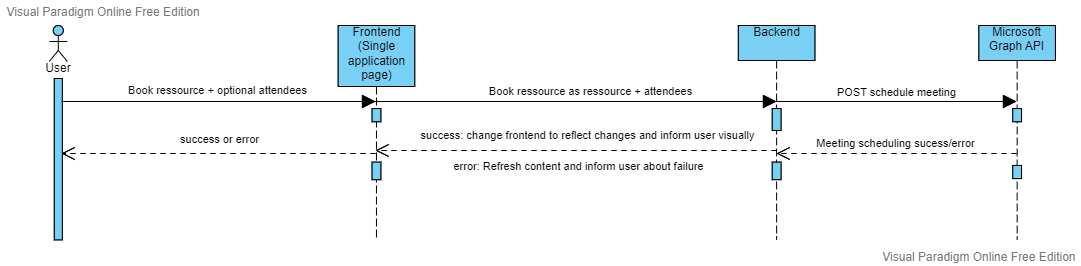
\includegraphics[width=\textwidth]{Bilder/Objektorientiertes Design/Sequence diagram for ressource booking (3)}
\par\vspace{0.5cm}\label{fig:figure}
\end{figure}
\justifying
\newline
\newline
\subsection{Timer}\label{subsec:timer}
Der Timer, welcher die übrig bleibende Zeit bis zum Ende des jetzigen Termins anzeigt funktioniert, wie folgt:
\newline
\newline
Es wird die Zeit bis zum Ende den jetzigen Termin berechnet, ausgehend von der Zeit, die zum Anfang des jetzigen Termins vergangen ist, und in Millisekunden umgerechnet.
Dann wird eine sich drehende Animation erstellt, die für diese Dauer abläuft.
\newline
Da die Dauer angepasst werden kann, muss bei Datenänderungen geprüft werden, ob sich die Dauer verändert hat.
%Glossar local storage
\newglossaryentry{Local Storage}{name=Local Storage,description={Local Storage ist ein Speicherort, in Browsern, welcher Daten lokal speichert.}}
Die Daten dafür werden im~\gls{Local Storage} gespeichert.
Falls eine Änderung stattgefunden hat, wird die Animation neu berechnet.
Bei der Änderung werden, damit die Animation visuell nicht von vorne anfängt, die Animationsdauer und die vergangene Zeit als neue Animationsdauer aufaddiert und die vergangene Zeit als negative Animationsverzögerung gesetzt, damit die Animation visuell betrachtet dort ist, wo sie relativ zur neuen Dauer sein sollte.
\newline
\newline
Die Formel lautet, wie folgt:
\newline
\newline
\begin{equation}
\begin{aligned}
    \text{Vergangene Zeit} &= \text{Jetzt} - \text{Start} \\
\text{Animationsdauer} &= \text{Ende} - \text{Start} \\
    \text {Animationsverzögerung} &= \text{-Vergangene Zeit} \\
\end{aligned}\label{eq:equation}
\end{equation}
\newline
\newline
Die Berechnung wurde wie folgt implementiert:
\newline
\newline
\begin{lstlisting}[language=JavaScript,label={lst:JavaScript Timer}]
let currentEventBeginningTime = localStorage.getItem('currentEventBeginningTime');
let timePassed = (new Date() - new Date(currentEventBeginningTime + 'Z')) / 1000;
let animationDuration = ((new Date(currentEventEndTime + 'Z') - new Date(currentEventBeginningTime + 'Z')) / 1000);
firstHandSpan.style.animationDuration = animationDuration  + 's';
secondHandSpan.style.animationDuration = animationDuration + 's';
firstHandSpan.style.animationDelay = -timePassed + 's';
secondHandSpan.style.animationDelay = -timePassed  + 's';
\end{lstlisting}
\newline
\newline
Um die Animation während ihrer Laufzeit zu ändern, wird ein sogenannter Reflow ~\footcite{JavaScriptAnimationsReflow} erzwungen, indem die offsetWidth Eigenschaft abgefragt, die Animationsdauer und -verzögerung neu gesetzt und der Animationsname erst entfernt und dann wieder hinzugefügt wird.
\newline
\newline
\subsection{Persistente Datenspeicherung}\label{subsec:persistente-datenspeicherung}
Um die Daten der Anwendung zu speichern, wurde für kleinere Datensätze der Local Storage verwendet.
Dieser ist in jedem Browser verfügbar und darf bis zu 5 MB groß sein.
\newline
\newline
Für größere Datensätze wurde IndexedDB~\cite{IndexedDB} verwendet.
\newglossaryentry{caniuse}{name={caniuse.com},description={Caniuse is a website that shows you browser support for various features and includes references to the relevant specifications.}}
Dies ist eine NoSQL Datenbank, die in jedem gängigen Browser~\cite{caniuse-indexedDB} (\gls{caniuse}) verfügbar ist.
Die maximale Größe bei Chrome beträgt 80\(\%\) des verfügbaren Speichers.
Da es im Internet viele, sich widersprechende Angaben zu dieser Größe gibt, wurde diese manuell, mit folgendem Code, in der Konsole des Browsers, getestet:
\newline
\newline
\begin{lstlisting}[language=JavaScript,label={lst:JavaScript IndexedDB Speichergröße}]
    if (navigator.storage && navigator.storage.estimate) {
    const quota = await navigator.storage.estimate();
    // quota.usage -> Number of bytes used.
    // quota.quota -> Maximum number of bytes available.
    const percentageUsed = (quota.usage / quota.quota) * 100;
    console.log("You've used ${percentageUsed}% of the available storage.");
    const remaining = quota.quota - quota.usage;
    console.log("You can write up to ${remaining} more bytes.");
    }
\end{lstlisting}
\newline
\newline
Die Festplatte, auf der dies getestet wurde, hatte ca. 828 GB freien Speicher.
Das Ergebnis lautete, wie folgt:
\newline
\newline
\begin{lstlisting}[language=JavaScript,label={lst:JavaScript IndexedDB Speichergröße Ergebnis}]
    You've used 0.000002393592594674544% of the available storage.
    You can write up to 599726105785 more bytes.
\end{lstlisting}
\newline
\newline
%equation
\begin{equation}
    \begin{aligned}
       \text{verbleibender Speicher} &= \text{599726105785 Bytes}\\
       \newline
       \text{599726105785 Bytes} \text{ * 10}\textsuperscript{-9} &= \text{599,726105785 Gigabytes}\\
        \newline
        \newline
    \end{aligned}
\end{equation}
\newline
\newline
Das sind etwas über 70 \%\) der verfügbaren Speicherkapazität.
Hier ist davon auszugehen, dass die restlichen 10 \%\) für andere Daten schon verwendet werden.
Zudem ist zu betrachten, dass die \"\).\"\) Schreibweise für Dezimalzahlen in JavaScript verwendet wurde, während wiederum die \"\),\"\) Schreibweise für die mathematische Gleichung verwendet wurde.
Dies hat den Hintergrund, dass die \"\),\"\) Schreibweise in JavaScript nicht grundsätzlich unterstützt wird, beziehungsweise, die Konvention beim Programmieren verlangt, dass man auf Englisch programmiert und im Englischen die Dezimalzahlen mit einem Punkt geschrieben werden.
\newline
\newline
Die Datenbank befindet sich aufgrund ihrer geringen Komplexität in der 5. Normalform.
Der Schlüssel besteht aus dem Namen der Firma, zu der, das Logo gehört und gibt das nicht Primärattribut zurück, welches das Bild, in Base64, enthält.
Schlüssel müssen eindeutig sein.
IndexedDB unterstützt die Eigenschaft \"\)unique\"\), welche dafür sorgt, dass der Schlüssel eindeutig ist.
Jedoch gehen wir auch manuell noch einmal sicher, dass der Schlüssel eindeutig ist, also dass sich dieser, noch nicht in der Datenbank befindet.
Eine weitere Aufteilung würde zu Informationsverlust führen, da der Firmenname eindeutig ist.
\newline
\newline
Zwar gibt es die Möglichkeit die Bilder für Firmen, zu updaten, welcher der User auch so wahrnimmt, jedoch wird der Schlüssel des alten Bildes entfernt und ein neuer Schlüssel mit dem neuen Bild hinzugefügt.
Dies ist notwendig, da der Schlüssel eindeutig sein muss.
Somit löschen wir den alten Eintrag und fügen einen neuen hinzu.
Unabhängig von der Interaktion mit der Datenbank, wird sichergestellt, dass sinnfreie Anfragen an die Datenbank nicht gesendet werden.
Falls der User beispielsweise ein Bild hochlädt, welches bereits in der Datenbank, für genau den gleichen Schlüssel, vorhanden ist, wird die Anfrage an die Datenbank nicht gesendet oder falls der User versucht ein Bild aus der Datenbank zu entfernen, welches gar nicht existiert.
\newline
\newline
%Tabelle erläutern
\subsection{Azure Authentifizierung}\label{subsec:Azure Authentifizierung}
Um die Authentifizierung zu realisieren, wurden folgende Berechtigungen benötigt:
\newline
\newline
%    \begin{table}
    \centering
%table should not be wider than 0.8\textwidth
\small
    \begin{tabularx}{\textwidth}{|X|X|X|}
        \toprule
        \textbf{Calendars.Read} & \textbf{Delegiert} & \textbf{Lesezugriff auf Benutzerkalender}\\
        \midrule
        Calendars.Read.Shared & Delegiert & Benutzer und freigegebene Kalender lesen\\
        Calendars.ReadWrite & Delegiert & Verfügt über Vollzugriff auf Benutzerkalender.\\
        Calendars.ReadWrite.Shared & Delegiert & Benutzerdefinierte und freigegebene Kalender lesen und schreiben\\
        email & Delegiert & E-Mail-Adresse von Benutzern anzeigen \\
        IMAP.AccessAsUser.All & Delegiert & Read and write access to mailboxes via IMAP.\\
        Mail.Read & Delegiert & Lesezugriff auf Benutzer-E-Mails\\
        Mail.Send & Delegiert & E-Mails unter einem anderen Benutzernamen senden\\
        Mail.Send.Shared & Delegiert & E-Mails im Namen anderer Benutzer senden\\
        offline\_access & Delegiert & Zugriff auf Daten beibehalten, für die Sie Zugriff erteilt haben\\
        OnlineMeetings.Read & Delegiert & Read user's online meetings\\
        OnlineMeetings.ReadWrite & Delegiert & Read and create user's online meetings\\
        openid & Delegiert & Benutzer anmelden\\
        profile & Delegiert & Grundlegendes Profil von Benutzern anzeigen\\
        User.Read & Delegiert & Anmelden und Benutzerprofil lesen\\
        \bottomrule
    \end{tabularx}
    \caption{}
    \label{tab:}
%    \end{table}
\newline
\newline
\raggedright
\normalsize
Diese werden beim erstmaligen Login, vom User, seitens Microsoft, angefordert.
Ohne die Zustimmung des Users, wird die Anwendung nicht entsprechend den Anforderungen, funktionieren und wird weiterhin darauf hinweisen, dass der User sich anmelden soll.
